\documentclass{article}
\usepackage{natbib, graphicx,xspace}
\long\def\comment#1{\xspace}
\begin{document}
\title{Illuminating poverty: Using satellite light detection for a poverty indicator}
\maketitle
\begin{abstract}
Satellite data includes areas that are difficult to reach via surveys or traditional big
data sources like cash registers and computers. We consider the use of luminosity data
from space as a correlate to poverty, using data from Bangladesh and Guatemala.
\end{abstract}

\section{Introduction}

Measuring poverty is a famously difficult problem: the poor and disadvantaged tend to be
hard-to-reach by survey or census takers \citep{h2r:asa}, and thus require far greater resources to
survey. Conversely, satellite data is readily available and consistently taken
regardless of the social standing of the population being observed. 



\citet{chen:pnas} and \citet{henderson:nber} wrote on using luminosity as a measure of GDP.
However, GDP and poverty are very imperfectly correlated.

\section{Data} We use data from NOAA measuring the mean night-time intensity of light in
the visible light range. The smallest resolution, one pixel in our data, covers about
30 arc seconds of earth, which is approximately one square kilometer at the Equator. For comparison,
the capital city of Bangladesh (Dhaka) is 360 km$^2$, and the capital district of the
United States (Columbia) is 177 km$^2$. Each pixel of data has an intensity from zero
to 63.

This is a notably smaller scale than prior efforts at matching socioeconomic and satellite
data, such as Yale University's G-Econ program, which works at a $1^\circ$ resolution.
The NOAA data provides 144 pixels in each $1^\circ \times 1^\circ$ box.

The full area of Bangladesh (147,570 km$^2$) was covered in 177,691 pixels. In 2001,
105,774 (59.5\%) of the pixels were at zero intensity; in 2005, 108,551 pixels (61.0\%)
were at zero. In 2001, 100 pixels ($<$0.1\%) were at the maximum intensity of 63, and in
2005, 103 pixels were at the maximum intensity.
\comment{
Here's the shell script (should work on GNU \& Mac) BK used to produce the stats in the next column. Uses the database produced in the regress directory.
%  for yr in 2001 2005; do 
%      rm pixct
%      for i in `seq 0 63`; do sqlite3 b.db "select sum(year_${yr}_num_intensity_$i) from pandl" >>pixct; done
%      echo -n total px for $yr: 
%      awk '{sum+=$1;} END { print sum}' < pixct
%      echo -n zero px for $yr: 
%      sed -n '1p' < pixct
%      echo -n 64 px for $yr: 
%      sed -n '64p' < pixct
%  done
%  rm pixct
}


{\bf More on the intensity data here?}

{\bf How was the data divided into counties?}


{\bf Something here about the poverty measure from the Bangladeshi census}



\section{Model and methods}

Consider a set of $N$ agents, each of whom could produce a light source. The odds of
producing a light source are a function of availability of electricity, urbanization, and poverty.

Light intensity is additive: given one source producing $L_1$ candelas of light, and a
second producing $L_2$ candelas, the total luminosity observed is simply $L_1+L_2$.

We think light intensity is Lognormally distributed.
We found the Kullback-Leibler divergence between a true
Lognormal distribution and the histogram of data was good.
 {\bf Kolmogorov-Smirnov test of this
claim here.} We therefore summarize the luminosity in a district as 

$$\mu\ln L = \frac{\sum_j \ln(I_j)}{A},$$

where $I_j$ is the intensity (between 1 and 64) for pixel $j$, and $A$ is the total count
of pixels in the region.

Because we have luminosity data for
every year from 2001 to 2005, we can also make use of the change in $\mu\ln L$ over the given period.

All this will wind up with a form suitable for regression 

\[
\mu\ln L_i = \beta_{l0} + \beta_{l1} Pv + \beta_{l2} El + \beta_{l3} Ur + \epsilon_l,
\]

where $Pv$ is our poverty measure, $El$ is electrification, $Ur$ is urbanization.
We can rewrite this as 

\[\label{povertyregression}
Pv = \pi_0 + \pi_1 \mu\ln L_i  + \pi_2 El + \pi_3 Ur + \epsilon,
\]

where 
\begin{eqnarray*}
\pi_0 &=& -\beta_{l0}/\beta_{l1} \\
\pi_1 &=& 1/\beta_{l1} \\
\pi_2 &=& -\beta_{l2}/\beta_{l1} \\
\pi_3 &=& -\beta_{l3}/\beta_{l1} \\
    &\hbox{and}\\
\epsilon &=& \epsilon_l/\beta_{l1} \\
\end{eqnarray*}


\section{Results}
There is a correlation between log mean luminosity and density, urbanization, electric access, and
poverty, as shown in Figure \ref{corr}. 

{\bf Need confidence intervals? These are $\chi^2$ distributed, right?}

\begin{figure}
\begin{center}
\hrule
\begin{tabular}{lrrrrrrr}
& poverty        &   $\mu\ln$  &    $\Delta\mu\ln$ &  pop density &   \% electric & \% urban \\
poverty        &   1 & -0.351&  -0.352&        -0.111&    -0.544& 0.0467\\
$\mu\ln$       & -0.351&     1  &   0.434&       0.198&    0.840& 0.0413\\
$\Delta\mu\ln$ & -0.352&  0.434&    1 &         0.154&    0.463&0.0687\\
density    & -0.111&  0.198&   0.154&           1 &    0.231& 0.0536\\
\% electric     & -0.544&   0.84&  0.463 &        0.231&      1    &  0.262\\
\% urban       & 0.0467& 0.0413&  0.068&       0.0536&     0.262&     1
\end{tabular}
\hrule
\end{center}
\caption{Correlation coefficients.}\label{corr}
\end{figure}

The regression results for Equation \label{povertyregression} are displayed in Figure
\ref{regfig}. 
Our key concern is the coefficient on log mean luminosity, which a 2.6\%
decrease in poverty for every one-unit increase in log mean luminosity. The coefficient is
significantly different from zero with 99.3\% confidence.

{\bf BK: get your act together and discuss the conversion from the luminosity equation
to the poverty equation. Also, add robustness tests---it's too easy to respecify this
regression and get different results.}

\begin{figure}
\begin{center}
\hrule
\begin{tabular}{lrl}
                          & parameters&(pval)\\
constant                  & 0.485&(0)       \\
$\mu\ln$ luminosity       &-0.0262&(0.007)        \\
$\Delta\mu\ln$ luminosity & 0.0651&(0.0048)        \\
density                   & 0.0161&(0.25)        \\
pct electric              &-0.003299&(0)        \\
pct urban                 & 0.000790&(0.024)        
\end{tabular}
\hrule
\end{center}
\caption{Regression coefficients for a regression with poverty as the dependent variable.}\label{regfig}
\end{figure}

\begin{figure}
\begin{center}
%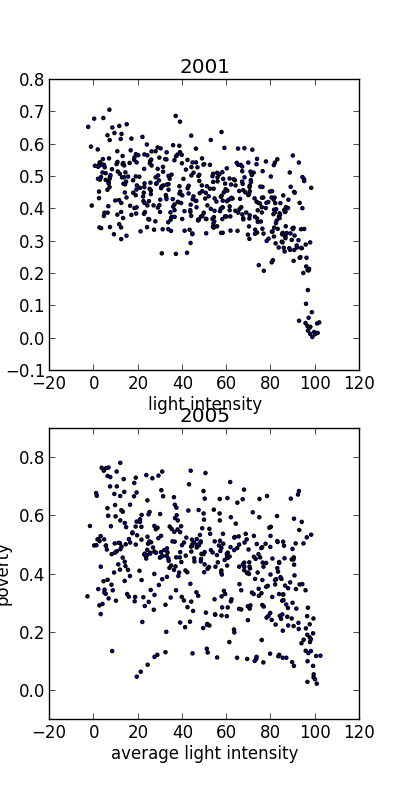
\includegraphics[width=\textwidth*\real{0.8}]{dotplot.png}
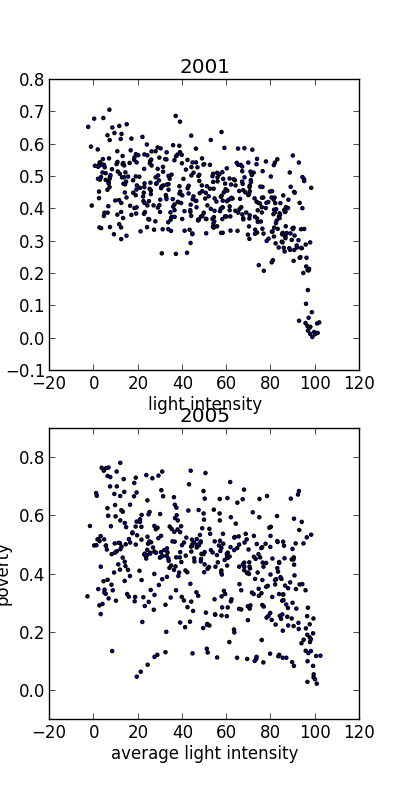
\includegraphics[width=7cm]{dotplot.png}

\end{center}
\caption{Scatterplot of light and poverty.}
\end{figure}

{\bf Here are some extremely attractive maps to get the point across.}

\section{Conclusion} We found that satellite luminosity data is correlated to poverty and
has some predictive power, even controlling for other factors. 
Luminosity is therefore one more tool available to researchers who hope to develop area-level
measures and predictions of poverty levels.

\bibliographystyle{plainnat}
\bibliography{luminosity}

\end{document}
